
\begin{figure}
    % \centering
    % \begin{subfigure}[c]{1.0\textwidth}
        \centering        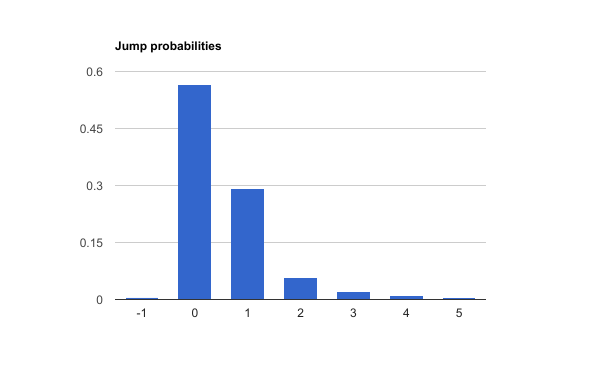
\includegraphics[scale=0.7]{resources/jump_distribution.png}
        \caption{The jump probability calculated from the training set and main test set.
        As expected, the following page is most likely the same year or the consecutive year. With laplace smoothing of $0.5$, the probability for a zero-transition is $56.5\%$ and the probability for a plus-one-transition is $29.1\%$. The interval $[-1,5]$ contains $95.5\%$ of the smoothed distribution.}
        \label{fig:jump_prob}
    % \end{subfigure}
    % \begin{subfigure}[c]{1.0\textwidth}
    %     \centering
    %     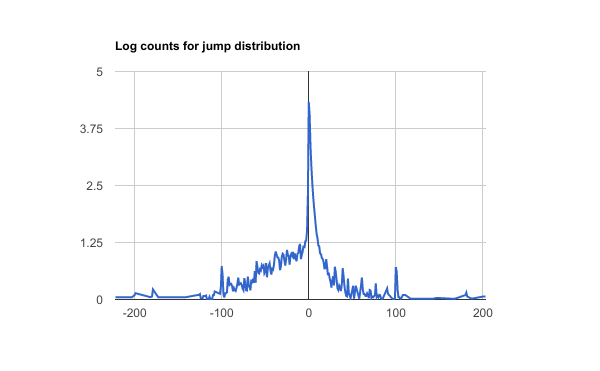
\includegraphics[scale=0.7]{resources/jump_log_counts.png}
    %     \caption{The plot shows $\log(1+\text{count}(x))$ for each label transition $x$.}
    %     \label{fig:jump_log_counts}
    % \end{subfigure}
    % \caption{The jump probability calculated from the training set and main test set.}
\end{figure}
